\documentclass[a4paper,10pt]{article}

% --- PACHETE DE BAZĂ (Ordinea este importantă!) ---
\usepackage[utf8]{inputenc}
\usepackage[T1]{fontenc}
\usepackage[romanian]{babel}
\usepackage[margin=2cm]{geometry}
\usepackage{amsmath, amssymb}
\usepackage{xcolor}

% --- PACHETE GRAFICE ---
% "babel" este vital aici pentru a preveni erorile specifice limbii române în desene
\usepackage{tikz}
\usetikzlibrary{babel, arrows, positioning, shapes}

% --- PACHETE PENTRU CUTII (BOXES) ---
\usepackage{tcolorbox}
\tcbuselibrary{skins, breakable}

% --- CULORI ---
\definecolor{mainblue}{RGB}{0, 60, 120}
\definecolor{conceptbg}{RGB}{240, 248, 255}
\definecolor{codebg}{RGB}{250, 250, 250}

% --- DEFINIȚII CUTII ---
\newtcolorbox{intuition}[1][]{
    colback=conceptbg, 
    colframe=mainblue!50, 
    title=\textbf{Intuiție / Logica din spate}, 
    coltitle=black, 
    fonttitle=\bfseries,
    breakable,
    #1
}

\newtcolorbox{algorithmbox}[1]{
    colback=codebg, 
    colframe=gray, 
    title=\textbf{Algoritm: #1}, 
    coltitle=black,
    fonttitle=\bfseries,
    breakable
}

\title{\textbf{Manual Complet de Teoria Grafurilor}}
\author{Sinteză Extinsă}
\date{}

\begin{document}

\maketitle
\tableofcontents
\newpage

% =========================================================
\section{1. Structura și Conexitatea}
% =========================================================

\subsection{Algoritmul Havel-Hakimi}

\begin{intuition}
Gândește-te la gradele nodurilor ca la niște "brațe" libere. Algoritmul spune: "Ia nodul cu cele mai multe brațe (șeful) și conectează-l cu următorii cei mai dotați". Dacă rămâi cu brațe negative (imposibil), nu se poate forma graful.
\end{intuition}

\begin{algorithmbox}{Havel-Hakimi}
Problema: Se dă o secvență de grade $S$. Putem construi un graf simplu?
\begin{enumerate}
    \item Sortează secvența descrescător: $d_1 \ge d_2 \ge \dots \ge d_n$.
    \item Dacă $d_1 > n-1$ sau apare un număr negativ $\to$ IMPOSIBIL.
    \item Dacă toate sunt $0$ $\to$ POSIBIL (STOP).
    \item Elimină $d_1$. Scade câte 1 din următoarele $d_1$ numere din listă.
    \item Repetă de la pasul 1.
\end{enumerate}
\end{algorithmbox}

\subsection{Parcurgeri: DFS vs BFS}
\begin{itemize}
    \item \textbf{BFS (Lățime):} Ca o undă într-un lac. Găsește cel mai scurt drum (ca număr de muchii). Folosește o \textbf{Coadă}.
    \item \textbf{DFS (Adâncime):} Ca un explorator într-un labirint care merge până se lovește de un zid, apoi se întoarce puțin (backtracking). Folosește o \textbf{Stivă}.
\end{itemize}

\subsection{Clasificarea Muchiilor în DFS}
Când parcurgem graful în adâncime, muchiile care NU fac parte din arborele DFS ne spun lucruri despre structura grafului.

\begin{center}
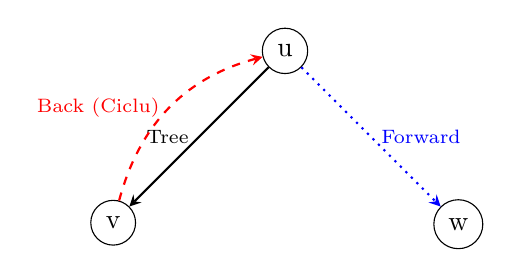
\begin{tikzpicture}[>=stealth, node distance=2.5cm]
    \node[circle, draw] (u) {u};
    \node[circle, draw] (v) [below left=of u] {v};
    \node[circle, draw] (w) [below right=of u] {w};
    
    % Muchii simple, fara stiluri complexe
    \draw[->, thick] (u) -- node[left, font=\scriptsize]{Tree} (v);
    \draw[->, dashed, red, thick] (v) to[bend left] node[left, red, font=\scriptsize]{Back (Ciclu)} (u);
    \draw[->, dotted, blue, thick] (u) -- node[right, blue, font=\scriptsize]{Forward} (w);
\end{tikzpicture}
\end{center}

\begin{intuition}
\begin{itemize}
    \item \textbf{Tree Edge:} Drumul normal pe care îl descoperim.
    \item \textbf{Back Edge (Roșu):} O "scurtătură" înapoi spre un strămoș. \textbf{Aceasta demonstrează existența unui CICLU.}
\end{itemize}
\end{intuition}

\subsection{Componente Tare Conexe (Kosaraju)}

\begin{intuition}
Ideea genială: Dacă poți ajunge de la A la B, și în graful cu sensurile inversate poți ajunge tot de la A la B (care de fapt e B la A în original), înseamnă că există un ciclu A-B-A.
\end{intuition}

\begin{algorithmbox}{Kosaraju (Complexitate V+E)}
\begin{enumerate}
    \item Fă DFS pe graful $G$ și reține nodurile într-o \textbf{stivă} în ordinea finalizării.
    \item Construiește graful transpus $G^T$ (inversează toate săgețile).
    \item Extrage nodurile din stivă. Dacă nodul curent nu e vizitat, pornește un nou DFS în $G^T$.
    \item Toate nodurile atinse într-un astfel de DFS formează o Componentă Tare Conexă (CTC).
\end{enumerate}
\end{algorithmbox}

\subsection{Muchii Critice (Punți)}
O muchie $(u, v)$ e critică dacă e singura cale de a ajunge la $v$ (eliminarea ei rupe conexitatea).

\begin{algorithmbox}{Detecție Muchii Critice}
Calculăm pentru fiecare nod $u$:
\begin{itemize}
    \item $niv[u]$: Nivelul în arborele DFS.
    \item $low[u]$: Cel mai mic nivel la care se poate ajunge folosind o muchie de întoarcere din subarborele lui $u$.
\end{itemize}
\textbf{Condiție:} Muchia $(u,v)$ este critică dacă $low[v] > niv[u]$ (adică din $v$ nu te poți întoarce "mai sus" de $u$).
\end{algorithmbox}

% =========================================================
\section{2. Arbori Parțiali de Cost Minim (APCM)}
% =========================================================

\begin{intuition}
Scopul: Să conectăm toate orașele cu cost total minim de asfaltare (fără a crea cicluri inutile).
\end{intuition}

\subsection{Algoritmul Kruskal}
\begin{itemize}
    \item \textbf{Strategie:} "Lacom după muchii".
    \item Sortează toate muchiile crescător după cost.
    \item Iterează și adaugă muchia doar dacă nu unește două noduri care sunt deja în aceeași componentă (folosind \textit{Disjoint Sets} / Union-Find).
\end{itemize}

\subsection{Algoritmul Prim}
\begin{itemize}
    \item \textbf{Strategie:} "Lacom după vecini".
    \item Pornește dintr-un nod arbitrar (zona asfaltată).
    \item La fiecare pas, alege cea mai ieftină muchie care iese din zona asfaltată către un nod nevizitat.
    \item Folosește \textit{Priority Queue}.
\end{itemize}

% =========================================================
\section{3. Drumuri Minime}
% =========================================================

\subsection{Algoritmul Dijkstra}
\begin{intuition}
Funcționează ca apa care curge prin țevi: ajunge mai întâi la nodurile apropiate. Relaxează vecinii imediat.
\textbf{Limitare:} Nu funcționează corect dacă există muchii cu cost negativ!
\end{intuition}
\textbf{Relaxarea:} 
$$ \text{Dacă } d[u] + w(u,v) < d[v] \Rightarrow d[v] = d[u] + w(u,v) $$

\subsection{Algoritmul Bellman-Ford}
\begin{intuition}
Este mai lent, dar sigur. Relaxează \textit{toate} muchiile de $N-1$ ori.
Funcționează și cu costuri negative.
\end{intuition}
\textbf{Detecție Ciclu Negativ:} Dacă la pasul $N$ se mai poate face o relaxare, înseamnă că există un ciclu infinit de scădere a costului.

\subsection{Algoritmul Floyd-Warshall}
Programare dinamică. Calculează drumul minim între \textbf{oricare două noduri}.
$$ d[i][j] = \min(d[i][j], \quad d[i][k] + d[k][j]) $$
Unde $k$ este un nod intermediar permis.

% =========================================================
\section{4. Fluxuri și Cuplaje}
% =========================================================

\subsection{Flux Maxim (Max Flow)}
\begin{intuition}
Gândește-te la o rețea de țevi. Câtă apă intră în Sursă ($S$) trebuie să iasă în Destinație ($T$), respectând capacitatea țevilor.
\textbf{Teorema Min-Cut:} Dacă tai rețeaua în două (separând $S$ de $T$), capacitatea totală a țevilor tăiate (dinspre $S$ spre $T$) este egală cu fluxul maxim. Gâtuirea limitează sistemul.
\end{intuition}

\subsection{Algoritmul Edmonds-Karp}
\begin{algorithmbox}{Edmonds-Karp}
Este varianta Ford-Fulkerson în care alegem mereu drumul de ameliorare cu \textbf{cele mai puține muchii} (folosind BFS) în graful rezidual.
\begin{enumerate}
    \item Caută drum $S \to T$ în graful rezidual cu BFS.
    \item Calculează capacitatea minimă pe acel drum (cât flux putem împinge).
    \item Actualizează fluxul (adaugă pe muchia directă, scade pe cea inversă).
    \item Repetă până nu mai găsești drumuri.
\end{enumerate}
\end{algorithmbox}

\subsection{Cuplaj Maxim în Graf Bipartit}
\begin{intuition}
Problema "angajați pe posturi". Se rezolvă cu Flux Maxim:
\begin{itemize}
    \item Creează o \textbf{Super-Sursă} legată de toți angajații.
    \item Creează o \textbf{Super-Destinație} legată de toate posturile.
    \item Toate capacitățile sunt 1.
    \item Fluxul Maxim = Numărul Maxim de Perechi (Cuplaje).
\end{itemize}
\end{intuition}

\begin{center}
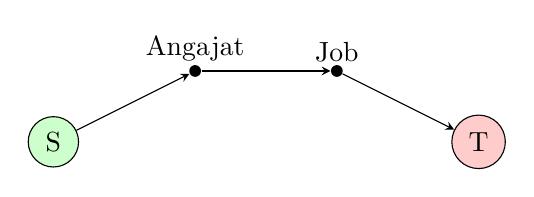
\begin{tikzpicture}[scale=0.9, >=stealth]
    % Noduri
    \node[draw, circle, fill=green!20] (S) at (0, 1.5) {S};
    \node[draw, circle, fill=red!20] (T) at (6, 1.5) {T};
    \node[circle, fill=black, inner sep=1.5pt] (u1) at (2, 2.5) {}; 
    \node[above] at (u1) {Angajat};
    \node[circle, fill=black, inner sep=1.5pt] (v1) at (4, 2.5) {}; 
    \node[above] at (v1) {Job};
    
    % Muchii
    \draw[->] (S) -- (u1); 
    \draw[->] (u1) -- (v1); 
    \draw[->] (v1) -- (T);
\end{tikzpicture}
\end{center}

% =========================================================
\section{5. Grafuri Speciale}
% =========================================================

\subsection{Eulerian vs Hamiltonian}
\begin{tcolorbox}[colback=white, title=Diferența Esențială]
\begin{itemize}
    \item \textbf{Eulerian (Muchii):} Vrei să parcurgi toate muchiile o singură dată (Poștașul).
    \item \textbf{Hamiltonian (Noduri):} Vrei să vizitezi toate orașele o singură dată (Comis-Voiajor).
\end{itemize}
\end{tcolorbox}

\begin{itemize}
    \item \textbf{Condiție Eulerian:} Graful să fie conex și toate nodurile să aibă \textbf{grad PAR}.
    \item \textbf{Condiție Hamiltonian:} Problemă grea (NP-Complet). \textit{Teorema Dirac:} Dacă $n \ge 3$ și orice nod are grad $\ge n/2$, atunci e Hamiltonian.
\end{itemize}

\subsection{Grafuri Planare}
Grafuri care pot fi desenate fără intersecții de muchii.
\textbf{Formula lui Euler:} $V - E + F = 2$ (unde $F$ include fața exterioară infinită).

% =========================================================
\section{6. Programare Dinamică: Distanța de Editare}
% =========================================================

\begin{intuition}
Cât ne costă să transformăm cuvântul "ANAF" în "BANANA"?
Putem: Șterge, Insera sau Înlocui o literă.
\end{intuition}

\begin{algorithmbox}{Recurența Levenshtein}
Fie $DP[i][j]$ costul pentru a transforma prefixul $A[1..i]$ în $B[1..j]$.
$$ DP[i][j] = \min \begin{cases} 
DP[i-1][j] + 1 & \text{(Ștergere)} \\
DP[i][j-1] + 1 & \text{(Inserare)} \\
DP[i-1][j-1] + cost & \text{(Substituție)}
\end{cases} $$
Unde $cost=0$ dacă literele sunt identice, și $1$ dacă sunt diferite.
\end{algorithmbox}

\end{document}